\section{Sharing and Contributing Code}

\begin{frame}[plain,noframenumbering]
 \vfill
 \begin{center}
  \LARGE \color{solarizedAccent} Sharing and Contributing Code
 \end{center}
 \vfill
\end{frame}

\begin{frame}[fragile]
 \frametitle{Sharing Code}

 \begin{itemize}
  \item Pushing commits only possible to \alert{bare} repositories (i.e.,
        GitHub, but not other clones) --- Must \textit{pull} from non-bare
        repositories
 \end{itemize}

 \begin{exampleblock}{Pushing Changes}
  \begin{semiverbatim}
\command{git push \only<2->{origin} \only<3->{master}\only<4->{:remote-name}}
Counting objects: 12, done.
Delta compression using up to 4 threads.
Compressing objects: 100% (9/9), done.
Writing objects: 100% (9/9), 1.80 KiB | 1 KB/s, done.
Total 9 (delta 6), reused 0 (delta 0)
To git@github.com:QuLogic/specfem3d_globe.git
   26ffb01..ab843d1  master -> master
\end{semiverbatim}
 \end{exampleblock}
\end{frame}

\begin{frame}
 \frametitle{Pull Requests}

 \begin{itemize}
  \item \alert{Pull Requests} indicate that you wish to merge changes from your
        fork into the Geodynamics repository
   \begin{tikzpicture}
    \node[anchor=south west, inner sep=0] at (0,0) {
     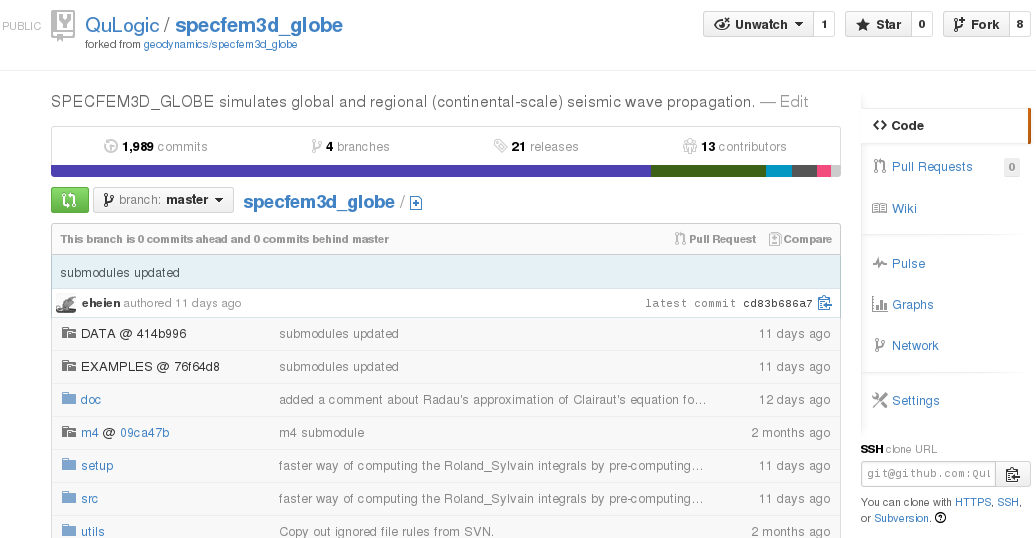
\includegraphics[width=\linewidth, height=\textheight, keepaspectratio,
                      trim={0 200px 0 100px}, clip]{github-fork}
    };
    \draw[solarizedAccent, thick, rounded corners]
     (6.5,0.8) rectangle (7.4,1.1);
   \end{tikzpicture}
  \item If available, set base branch to \alert{devel}
  \item Set head branch to feature branch in your fork or devel
 \end{itemize}
\end{frame}
